\documentclass[12pt,pdf,hyperref={unicode}]{beamer}
%\usetheme{boxes}
\beamertemplatenavigationsymbolsempty
\setbeamertemplate{footline}[page number]
% Set it for the internal PhD thesis defence to reduce number of slides
%\setbeamersize{text margin left=0.5em, text margin right=0.5em}

\usepackage[utf8]{inputenc}
%\usepackage[english, russian]{babel}
\usepackage{bm}
\usepackage{multirow}
\usepackage{ragged2e}
\usepackage{indentfirst}
\usepackage{multicol}
\usepackage{subfig}
\usepackage{amsmath,amssymb}
\usepackage{enumerate}
\usepackage{mathtools}
\usepackage{comment}
\usepackage[all]{xy}
\usepackage{tikz}
\usetikzlibrary{positioning,arrows}
\tikzstyle{name} = [parameters]
\definecolor{name}{rgb}{0.5,0.5,0.5}

%\usepackage{caption}
%\captionsetup{skip=0pt,belowskip=0pt}

%\newtheorem{theorem}{Theorem}
%\newtheorem{statement}{Statement}
%\newtheorem{definition}{Definition}

% colors
\definecolor{darkgreen}{rgb}{0.0, 0.2, 0.13}
\definecolor{darkcyan}{rgb}{0.0, 0.55, 0.55}
%\AtBeginEnvironment{figure}{\setcounter{subfigure}{0}}
%\captionsetup[subfloat]{labelformat=empty}

%----------------------------------------------------------------------------------------------------------

\title{LLMs Consistency in Describing and Scoring Personality}
\author{Danila Chernousov}
\institute[]{MIPT}
\date{2025}

%---------------------------------------------------------------------------------------------------------
\begin{document}
\begin{frame}
\titlepage
\end{frame}
\setcounter{page}{2}%remove here for the title
%----------------------------------------------------------------------------------------------------------
%\section{Please do not use sectioning in the presentations}
\begin{frame}
\frametitle{Goals}
\begin{itemize}
    \item Develop a framework for measuring LLM fidelity in personality profiling for any set of personality traits.
    \item Evaluate LLM consistency in converting numerical personality scores to text and back.
    \item Assess LLM performance on both well-established (e.g., Big Five) and understudied/synthetic traits.
    \item Investigate the impact of parameters (e.g., temperature) and trait ordering on consistency.
\end{itemize}
\end{frame}
%----------------------------------------------------------------------------------------------------------



\begin{frame}{LLMs consistency in personality scoring}

Experiment pipeline
	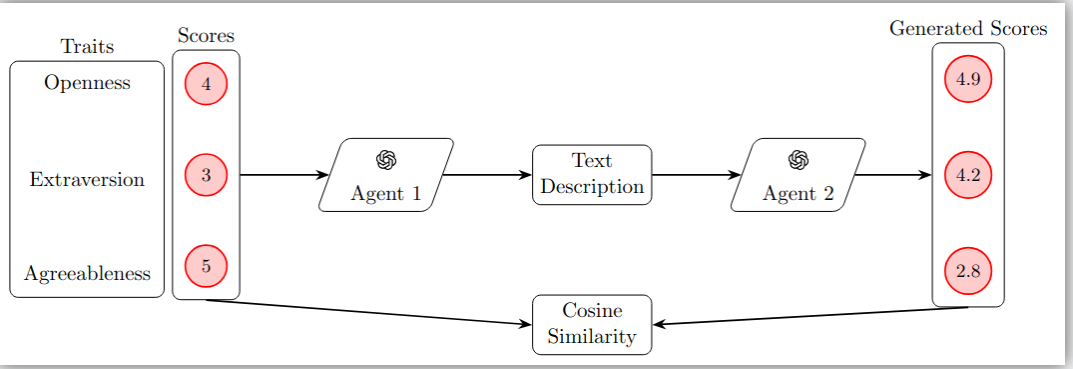
\includegraphics[width=1\textwidth]{Screenshot from 2025-03-27 01-49-06.png}  

\begin{enumerate}[1.]
    \item Big Five -- set of personality traits with a lot of research
    \item Personality conditioning -- prompting model with a personality
\end{enumerate}

     $S_{agent, traits}:$ score $\rightarrow$ text $ \ \ \ \ \ \ \ \ $$S_{agent, traits}^{-1}:$ text $\rightarrow$ score
    
\begin{center}
\textbf{Research question: $S(S^{-1}) = I$?}
\end{center}

\end{frame}

\begin{frame}{Literature}
Couple of motivational sentences
\begin{block}{The problem}
to investigate \ldots 
\end{block}
\begin{block}{The method needs a proper name here}
put the brief idea here
\end{block}
\begin{block}{The solution} your results appears twice, as a promise here and as a contribution later
\begin{enumerate}[1)]
\item set \ldots,
\item put \ldots,
\item get \ldots.
\end{enumerate}
\end{block}
\end{frame}


\begin{frame}
\frametitle{Evaluating LLM Consistency}
\begin{block}{Core Challenge}
\begin{itemize}
    \item LLMs lack intrinsic personality; their responses vary based on input structure (e.g., \textbf{trait order}, \textbf{prompt phrasing}).
    \item Prompting agent with personality induces consistency.
    \item No frameworks for evaluating LLMs along arbitrary personality dimensions 
\end{itemize}
\end{block}

\begin{block}{Key Questions}
\begin{itemize}
    \item Can LLMs reliably map between numerical scores (\textbf{p}) and textual descriptions (\textbf{d})?
    \item Is the reconstruction error $\|\mathbf{p} - g(f(\mathbf{p}))\| < \epsilon$ consistent across traits?
    \item Does error increase for understudied traits ($\mathcal{S} \subset \mathcal{P}$)?
\end{itemize}
\end{block}


\end{frame}



\begin{frame}{problem statement ends with quality criterion}
Couple of motivational sentences
\begin{block}{The problem}
to investigate \ldots 
\end{block}
\begin{block}{The method needs a proper name here}
put the brief idea here
\end{block}
\begin{block}{The solution} your results appears twice, as a promise here and as a contribution later
\begin{enumerate}[1)]
\item set \ldots,
\item put \ldots,
\item get \ldots.
\end{enumerate}
\end{block}
\end{frame}


\begin{frame}
\frametitle{Temperature Experiment: Key Findings}

\begin{columns}
\begin{column}{0.5\textwidth}
\textbf{Experimental Setup}
\begin{itemize}
    \item Varied temperature (0.2-1.5) during description generation
    \item 200 runs with Big Five traits
\end{itemize}

\vspace{0.3cm}
\textbf{Optimal Range Found}
\begin{itemize}
    \item Best balance at \textbf{T = 1.25}
    \item Preserves trait fidelity while allowing nuance
\end{itemize}
\end{column}

\begin{column}{0.7\textwidth}
\begin{figure}
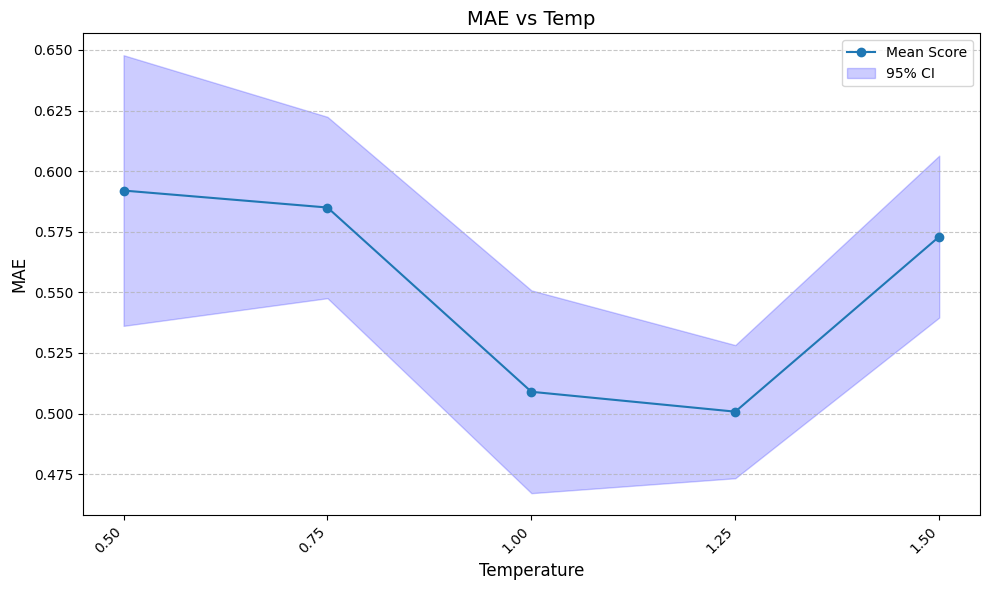
\includegraphics[width=\textwidth]{temp_dependency.png}
\caption{MAE vs. Temperature}
\end{figure}
\end{column}
\end{columns}

\begin{alertblock}{Key Insight}
Temperature isn't just stylistic - it \textbf{directly affects} how much latent trait signal survives text generation.
\end{alertblock}
\end{frame}


\begin{frame}
\frametitle{Ordering Experiment: Impact of Trait Sequence}

\begin{columns}
\begin{column}{0.5\textwidth}
\textbf{Experimental Design}
\begin{itemize}
    \item Tested 4 trait orderings with Big Five:
\end{itemize}

\vspace{0.8cm}
\textbf{Key Finding}
\begin{itemize}
    \item Order effect exists and is significant
\end{itemize}
\end{column}

\begin{column}{0.7\textwidth}
\begin{figure}
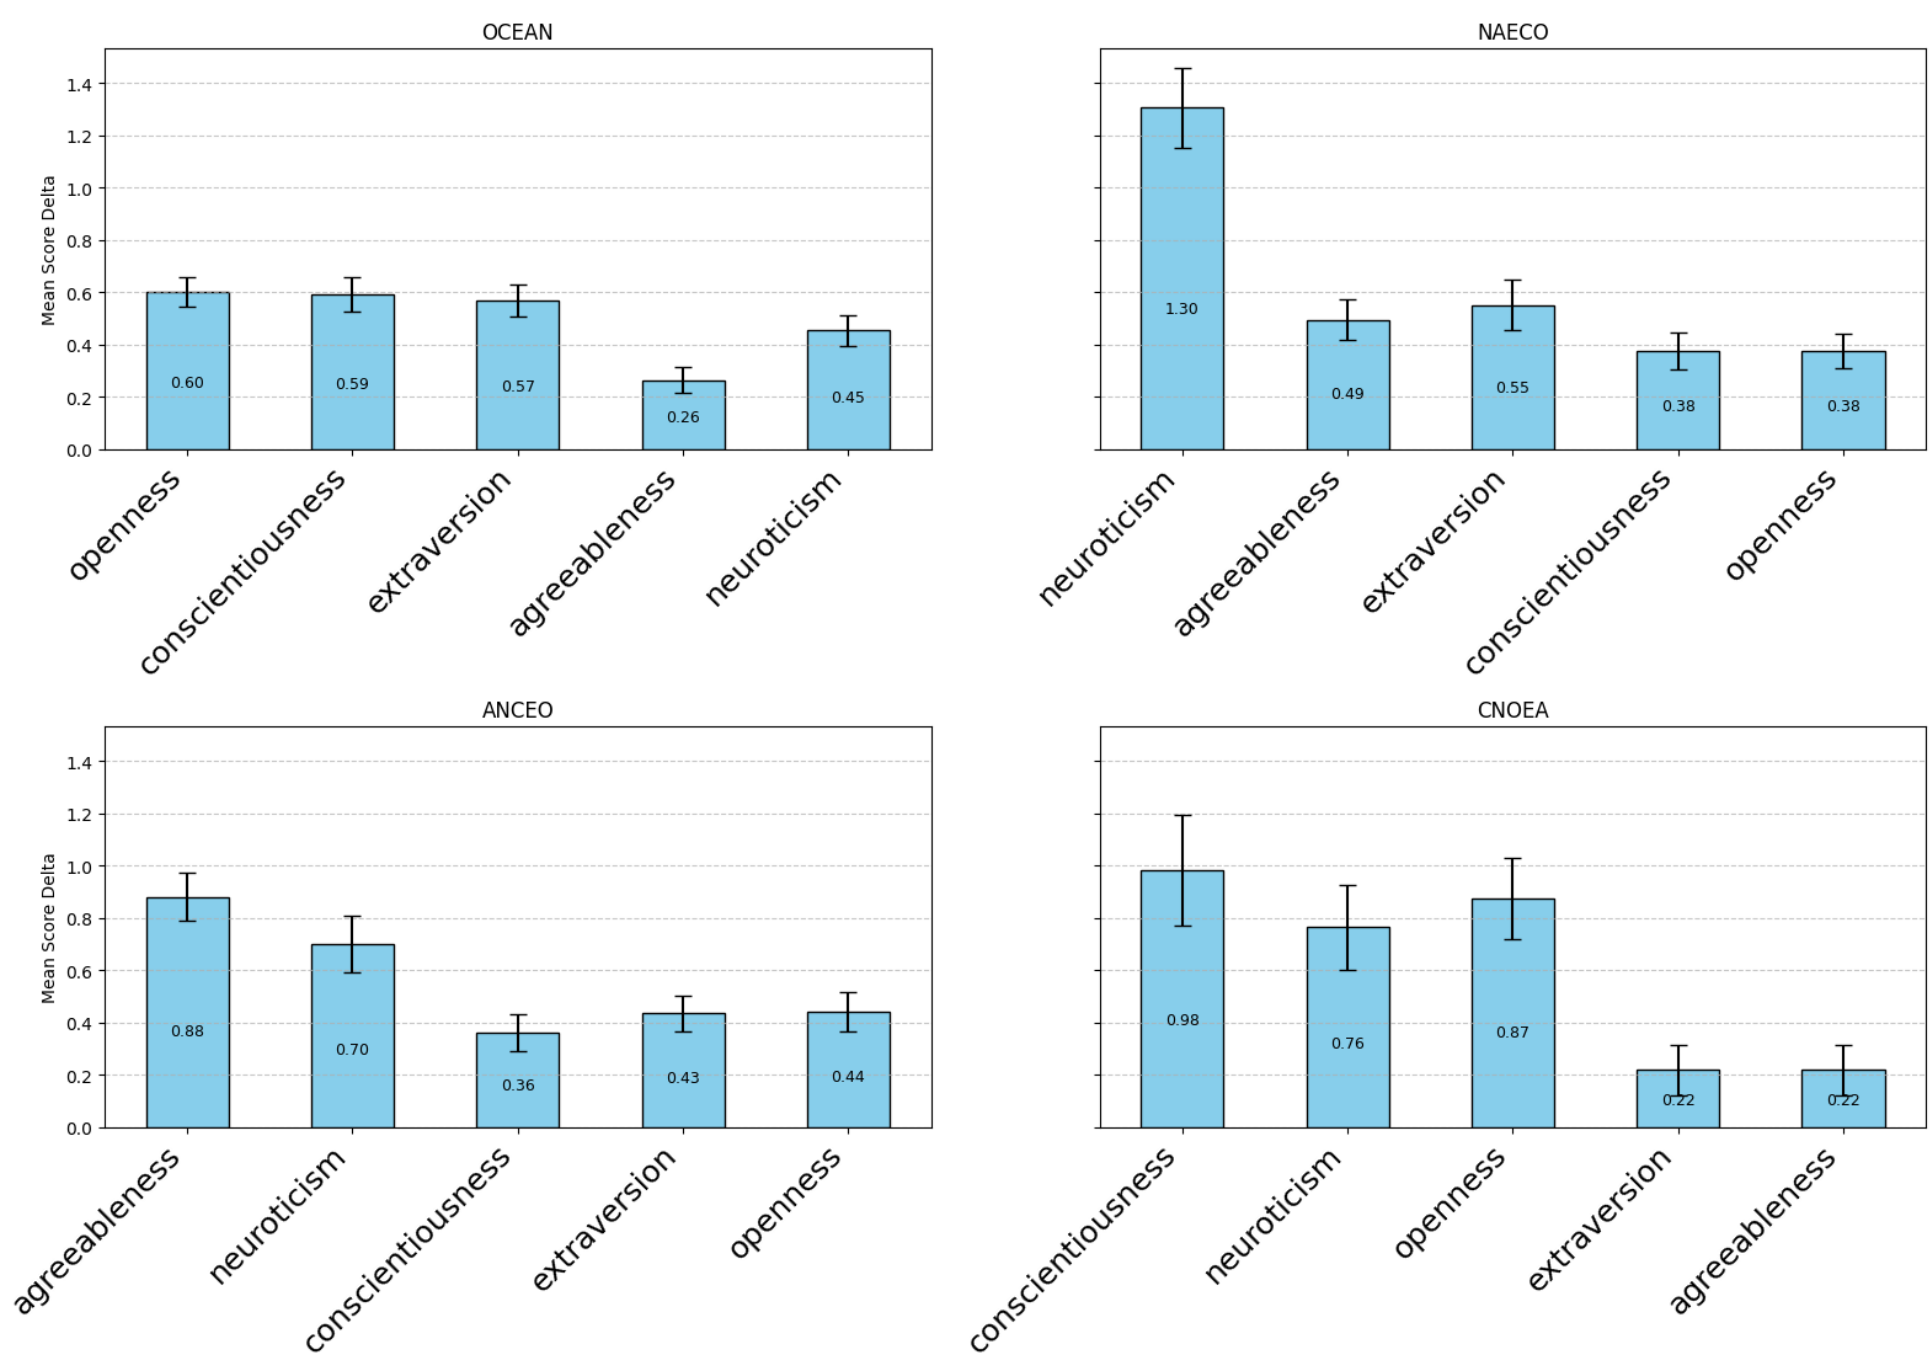
\includegraphics[width=\textwidth]{order_exp.png}
\caption{MAE across different trait orderings (O-C-E-A-N vs. alternatives)}
\end{figure}
\end{column}
\end{columns}
\end{frame}

\begin{frame}
\frametitle{Consistency Across Different Trait Sets}


\begin{columns}
\begin{column}{0.5\textwidth}
\textbf{Key Findings}
\begin{itemize}
    \item \textcolor{green}{Best performance} on Big Five (MAE 0.26-0.6)
    \item \textcolor{orange}{Moderate success} with clinical traits (MAE 0.4-1.2)
    \item \textcolor{red}{Highest errors} for synthetic traits (MAE up to 0.85)
\end{itemize}
\end{column}

\begin{column}{0.6\textwidth}
\begin{figure}
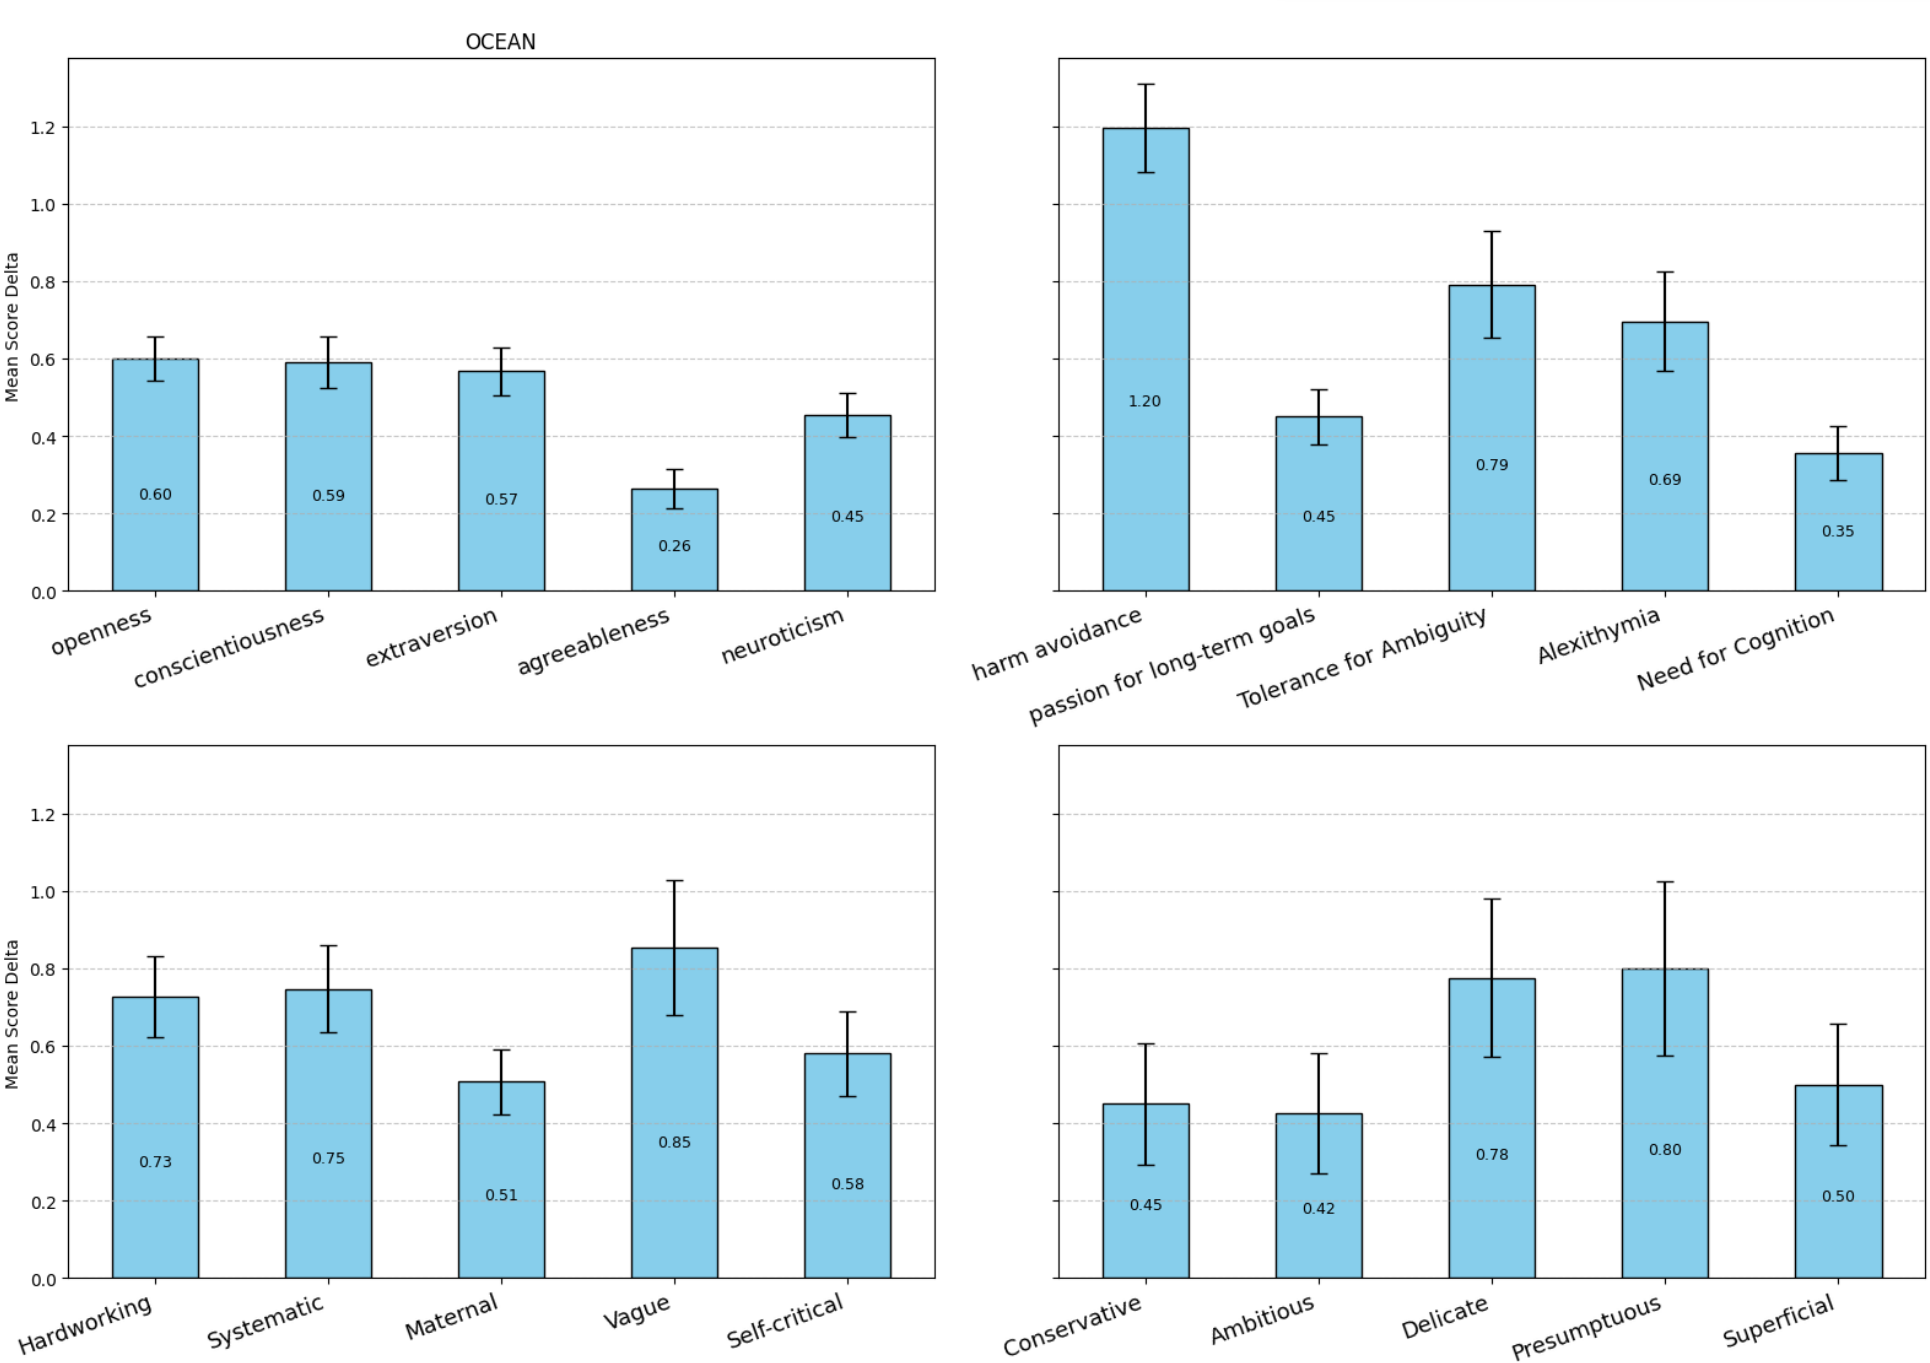
\includegraphics[width=\textwidth]{diff_traits.png}
\caption{MAE across trait categories (your Fig.4 data)}
\end{figure}
\end{column}
\end{columns}

\end{frame}


\begin{frame}
\frametitle{Conclusion \& Limitations}

\begin{block}{Key Findings}
\begin{itemize}
    \item \textbf{Two-stage framework} effectively measures LLM consistency in personality simulation
    \item \alert{Significant ordering effects}: Up to 11\% MAE variation across sequences
    \item Performance hierarchy:
    \begin{itemize}
        \item Big Five (best) $\gg$ Clinical traits $\gg$ Abstract/Synthetic
    \end{itemize}
\end{itemize}
\end{block}

\begin{block}{Limitations}
\begin{columns}
\begin{column}{0.5\textwidth}
\begin{itemize}
    \item Single-model bias (DeepSeekV3 only)
    \item Numerical MAE may mask semantic errors
\end{itemize}
\end{column}
\begin{column}{0.5\textwidth}
\begin{itemize}
    \item Ordering effects not tested on synthetic traits
\end{itemize}
\end{column}
\end{columns}
\end{block}

\end{frame}

\end{document}